\documentclass{beamer}
%
% Choose how your presentation looks.
%
% For more themes, color themes and font themes, see:
% http://deic.uab.es/~iblanes/beamer_gallery/index_by_theme.html
%
\mode<presentation>
{
  \usetheme{Darmstadt}      % or try Darmstadt, Madrid, Warsaw, ...
  \usecolortheme{crane} % or try albatross, beaver, crane, ...
  \usefonttheme{serif}  % or try serif, structurebold, ...
  \setbeamertemplate{navigation symbols}{}
  \setbeamertemplate{caption}[numbered]
} 

\usepackage[english]{babel}
\usepackage[utf8]{inputenc}
\usepackage[T1]{fontenc}



\def \calS{{\cal S}}
\def\mod#1{\llbracket{#1}\rrbracket}
\def \calF {\cal F}
\def \calB {\cal B}
\def \calT {\cal T}
\newcommand{\C}{\ensuremath{\mathbb C}}

 \def \dilT {\delta}
  \def \dilB {\presuper\calB\delta}
   \def \dilF {\presuper\calF\delta}
   

 %\def \erT {\presuper\calT\varepsilon}
 \def \erT {\varepsilon}
  \def \erB {\presuper\calB\varepsilon}
   \def \erF {\presuper\calF\varepsilon}
   
    \def \ordT {\preceq_{\calT}}
    \def \ordB {\preceq_{\calB}}
        \def \ordF {\preceq_{\calF}}

  %  \def \supT {\presuper\calT\vee}
   %     \def \infT {\presuper\calT\wedge}
        
        \def \supT {\vee}   
         \def \infT {\wedge}
    \def \supB {\presuper\calB\vee}
        \def \infB {\presuper\calB\wedge}
        \def \supF {\presuper\calF\vee}
                \def \infF {\presuper\calF\wedge}

    \def \supD {\presuper\calB\sqcup}
    \def \infD {\presuper\calB\sqcap}
  

 \def \LS{\mathcal{ALC(F)}} 
 \def \LSB{\mathcal{ALC(B)}} 
 

\newcommand{\EL}{\ensuremath{\mathcal EL}}
  


\newcommand{\Gr}{\ensuremath{\mathbf{Gr}}}


\newtheorem{algorithm}{Algorithme}
\newtheorem{defin}{D\'efinition}
\newtheorem{theor}{Th\'eor\`eme}
\newcommand{\ro}{\left[ o \right]}
\newcommand{\diam}{\langle o \rangle} 
\newcommand{\ra}{ \rightarrow} 
\newcommand{\lra}{ \leftrightarrow} 
\newcommand{\K}{{\cal{K}}}
\newcommand{\T}{{\cal{T}}}
\newcommand{\I}{{\cal{I}}}
\newcommand{\W}{{\cal{W}}}
\newcommand{\B}{{\cal{B}}}
\newcommand{\LL}{{\cal{L}}}
\newcommand{\A}{{\cal{A}}}

\def \calP{{\cal P}}
\def\expl#1#2{{#2}\rhd{#1}}
\newcommand{\Elc}[2]{{#2}\rhd^{\ell c}{#1}}
\newcommand{\Elne}[2]{{#2}\rhd^{\ell ne}{#1}}
\newcommand{\nElne}[2]{{#2}\not\!\!\rhd^{\ell ne}{#1}}
\newcommand{\iffdef}{\quad\!\!\stackrel{def}{\Leftrightarrow}\!\!\quad}
\newcommand{\BT}{{\cal{K}}}

\newcommand{\LLE}{\mbox{\sf LLE}}
\newcommand{\LLEs}{\mbox{\sf LLE$_{\scriptscriptstyle\Sigma}$}}
\newcommand{\LLEk}{\mbox{\sf LLE$_{\scriptscriptstyle\K}$}}
\newcommand{\RW}{\mbox{\sf RW}}
\newcommand{\REF}{\mbox{\sf REF}}
\newcommand{\OR}{\mbox{\sf OR}}
\newcommand{\AND}{\mbox{\sf AND}}
\newcommand{\CM}{\mbox{\sf CM}}
\newcommand{\RM}{\mbox{\sf RM}}
\newcommand{\DR}{\mbox{\sf DR}}
\newcommand{\RT}{\mbox{\sf RT}}

\def\nms{\vdash_{\scriptscriptstyle{\Sigma}}}
\def\RLE{\mbox{\sf RLE}}
\def\RLEs{\mbox{\sf RLE$_{\scriptscriptstyle\Sigma}$}}
\def\RLEk{\mbox{\sf RLE$_{\scriptscriptstyle\K}$}}
\def\con{\mbox{\sf Con$\boldmath {}_{\scriptscriptstyle\Sigma}$}}
\def\SRLE{\mbox{\sf RLE$_\Sigma$}}
\def\ECOMP{\mbox{\sf E-Comp}}
\def\Econ{\mbox{\sf E-Con$\boldmath {}_{\scriptscriptstyle\Sigma}$}}
\def\EconK{\mbox{\sf E-Con$\boldmath {}_{\scriptscriptstyle\K}$}}
\def\ECM{\mbox{\sf E-CM}}
\def\EWCM{\mbox{\sf E-W-CM}}
\def\EDR{\mbox{\sf E-DR}}
\def\EWDR{\mbox{\sf LOR}}
\def\WDR{\mbox{\sf W-DR}}
\def\RA{\mbox{\sf RS}}
\def\ECC{\mbox{\sf E-C-Cut}}
\def\EWCC{\mbox{\sf E-W-C-Cut}}
\def\ERC{\mbox{\sf E-R-Cut}}
\def\EWRC{\mbox{\sf E-W-R-Cut}}
\def\Ecut{\mbox{\sf E-Cut}}
\def\Edisj{\mbox{\sf E-Disj}}
\def\ERW{\mbox{\sf ROR}}
\def\ROR{\mbox{\sf ROR}}
\def\LOR{\mbox{\sf LOR}}
\def\ERef{\mbox{\sf E-Reflexivity}}
\def\ECONS{\mbox{\sf E-Cons}}
%\newcommand{\Gr}{\ensuremath{\mathbf{Gr}}}

\renewcommand{\Re}{\ensuremath{\mathbb{R}}}
\newcommand{\dataUni}{\ensuremath{y}}
\newcommand{\data}{\ensuremath{Y}}
\newcommand{\M}{m}
\newcommand{\N}{n}
\newcommand{\Vdim}{\ensuremath{\rho}}
\newcommand{\dicoUni}{\ensuremath{\phi}}
\newcommand{\dico}{\ensuremath{\Phi}}
\newcommand{\Coef}{\ensuremath{X}}
\newcommand{\coef}{\ensuremath{x}}
\newcommand{\DicoUni}{\ensuremath{U}}
%\newcommand{\dicoUni}{\ensuremath{u}}
\newcommand{\Dico}{\ensuremath{\mathbf{U}}}

\newcommand{\FLO}{\ensuremath{\mathcal{FL}_0}}
\newcommand{\ALEN}{\ensuremath{\mathcal{ALEN}}}
\newcommand{\ELext}{\ensuremath{\mathcal{ELU}}}
\newcommand{\ALC}{\ensuremath{\mathcal{ALC}}}
\newcommand{\ALCQ}{\ensuremath{\mathcal{ALCQ}}}

\newcommand{\NC}{\ensuremath{\mathcal{N}_C}}
\newcommand{\NR}{\ensuremath{\mathcal{N}_R}}



\title[GT IA]{Augmenting Transfer Learning with Semantic Reasoning}
\author{F. Lécué, J. Chen, J.Z. Pan, H. Chen}
\institute{IJCAI 2019}

\begin{document}

\begin{frame}
  \titlepage
\end{frame}

% Uncomment these lines for an automatically generated outline.
%\begin{frame}{Outline}
%  \tableofcontents
%\end{frame}

\section{Introduction}

\begin{frame}{Contexte}

\begin{block}{Transfer Learning}
\begin{itemize}
  \item Un domaine cible avec peu de données annotées
  \item Utilisation des données d'un domaine source \textbf{lié} pour apprendre un modèle de prédiction sur le domaine cible.
\end{itemize}
\end{block}
Questions :
\begin{itemize}
    \item Qu'est ce qui permet d'assurer un \textit{transfert positif} du domaine source vers le domaine cible ?
    \item Proposition :
    \begin{itemize}
        \item Représentation explicite de la sémantique des tâches d'apprentissage et des domaines source et cible.
        \item Augmenter la tâche de transfert avec de la sémantique.
    \end{itemize}
\end{itemize}
\end{frame}




\begin{frame}{Vue globale}
\begin{figure}
    \centering
    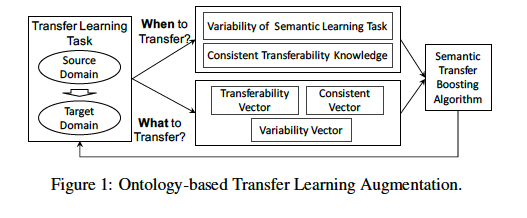
\includegraphics[scale=0.6]{Figures/vueglobale.png}
    \caption{Vue globale}
    \label{fig:my_label}
\end{figure}

\end{frame}

\section{State of the art}
\begin{frame}{Etat de l'art}

\begin{block}{Trois familles d'approches}
\begin{itemize}
    \item \textbf{Instance transfer (importance sampling)} : repondération d'instances du domaine source
    \begin{itemize}
    \footnotesize
        \item Ex : Distant Domain Transfer Learning, Tan et al, 2017
    \end{itemize}
    \item \textbf{Model Transfer} : réutilisation des paramètres du modèle appris sur le source
     \begin{itemize}
    \footnotesize
        \item Ex : Domain adaptation via tranfer component analysis, Pan et al, 2011
    \end{itemize}
    \item \textbf{Semantic transfer} : utilisation de connaissances a priori pour \textit{guider} le transfert.
    \begin{itemize}
    \footnotesize
        \item Knowledge Transfer with Interactive Learning of Semantic Relationships, Choi et al, AAAI 2016
        \item Transfer Learning for Deep Learning on Graph-Structured Data, Lee et al, AAAI 2017
        \item Avec des réseaux de markov logiques : TODTLER: Two-Order-Deep Transfer Learning, Van Haaren et al, AAAI 2015
    \end{itemize}
\end{itemize}
\end{block}

\end{frame}




\section[Background]{Background}




\begin{frame}
\frametitle{Descriptions logics}
	\begin{itemize}
	\footnotesize
\item Famille de logiques formelles pour représenter des informations structurées.
	\item Sémantique bien définie.
	\item Définies par un ensemble de concepts et des contructeurs de rôles.
	\item Compactes, expressives et bases du langage d'ontologie OWL.
	\end{itemize}	
\centerline{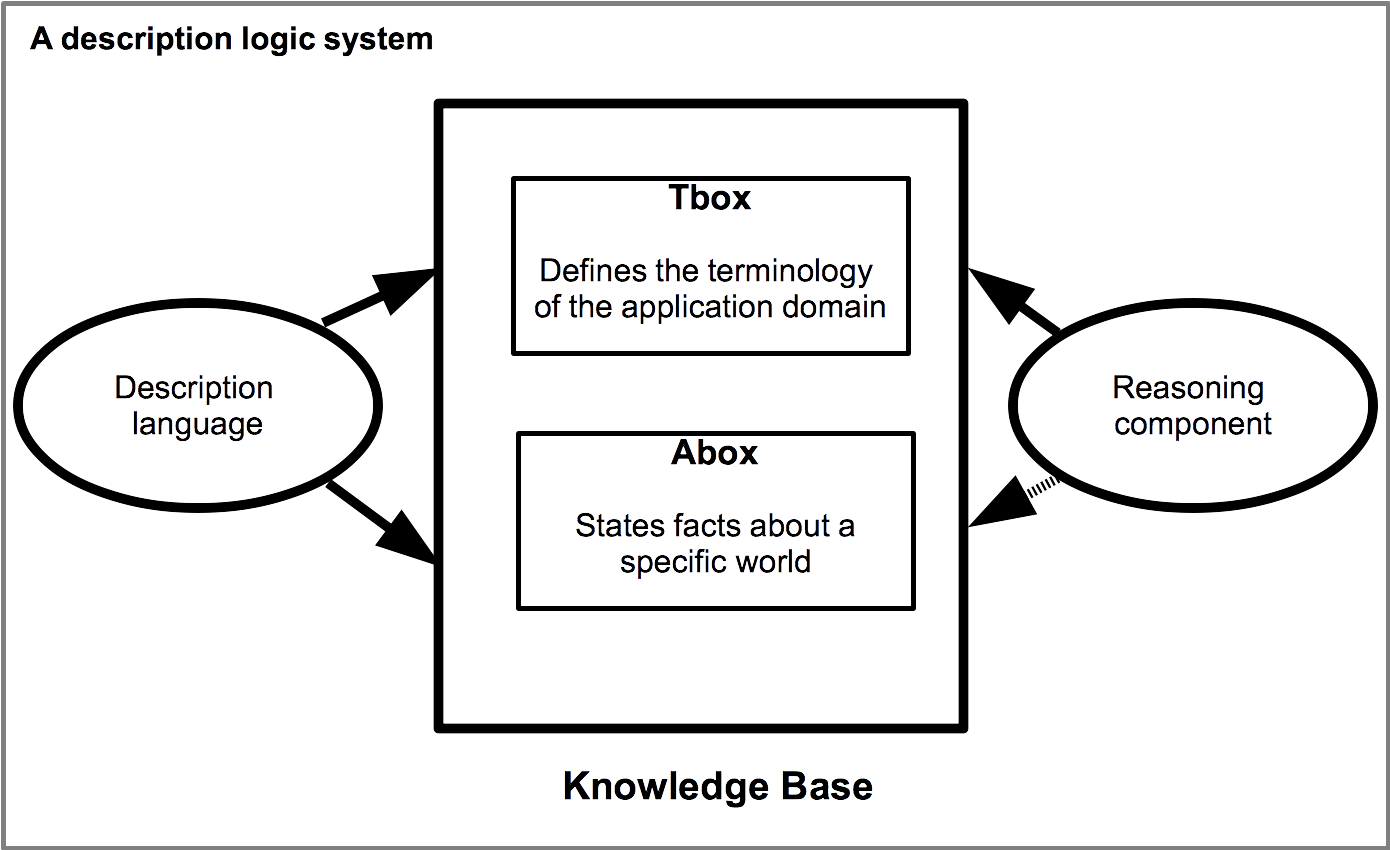
\includegraphics[scale=0.34]{./Figures/DLKB.png}}
	

\end{frame}



\begin{frame}
\frametitle{Descriptions logics}
\centering
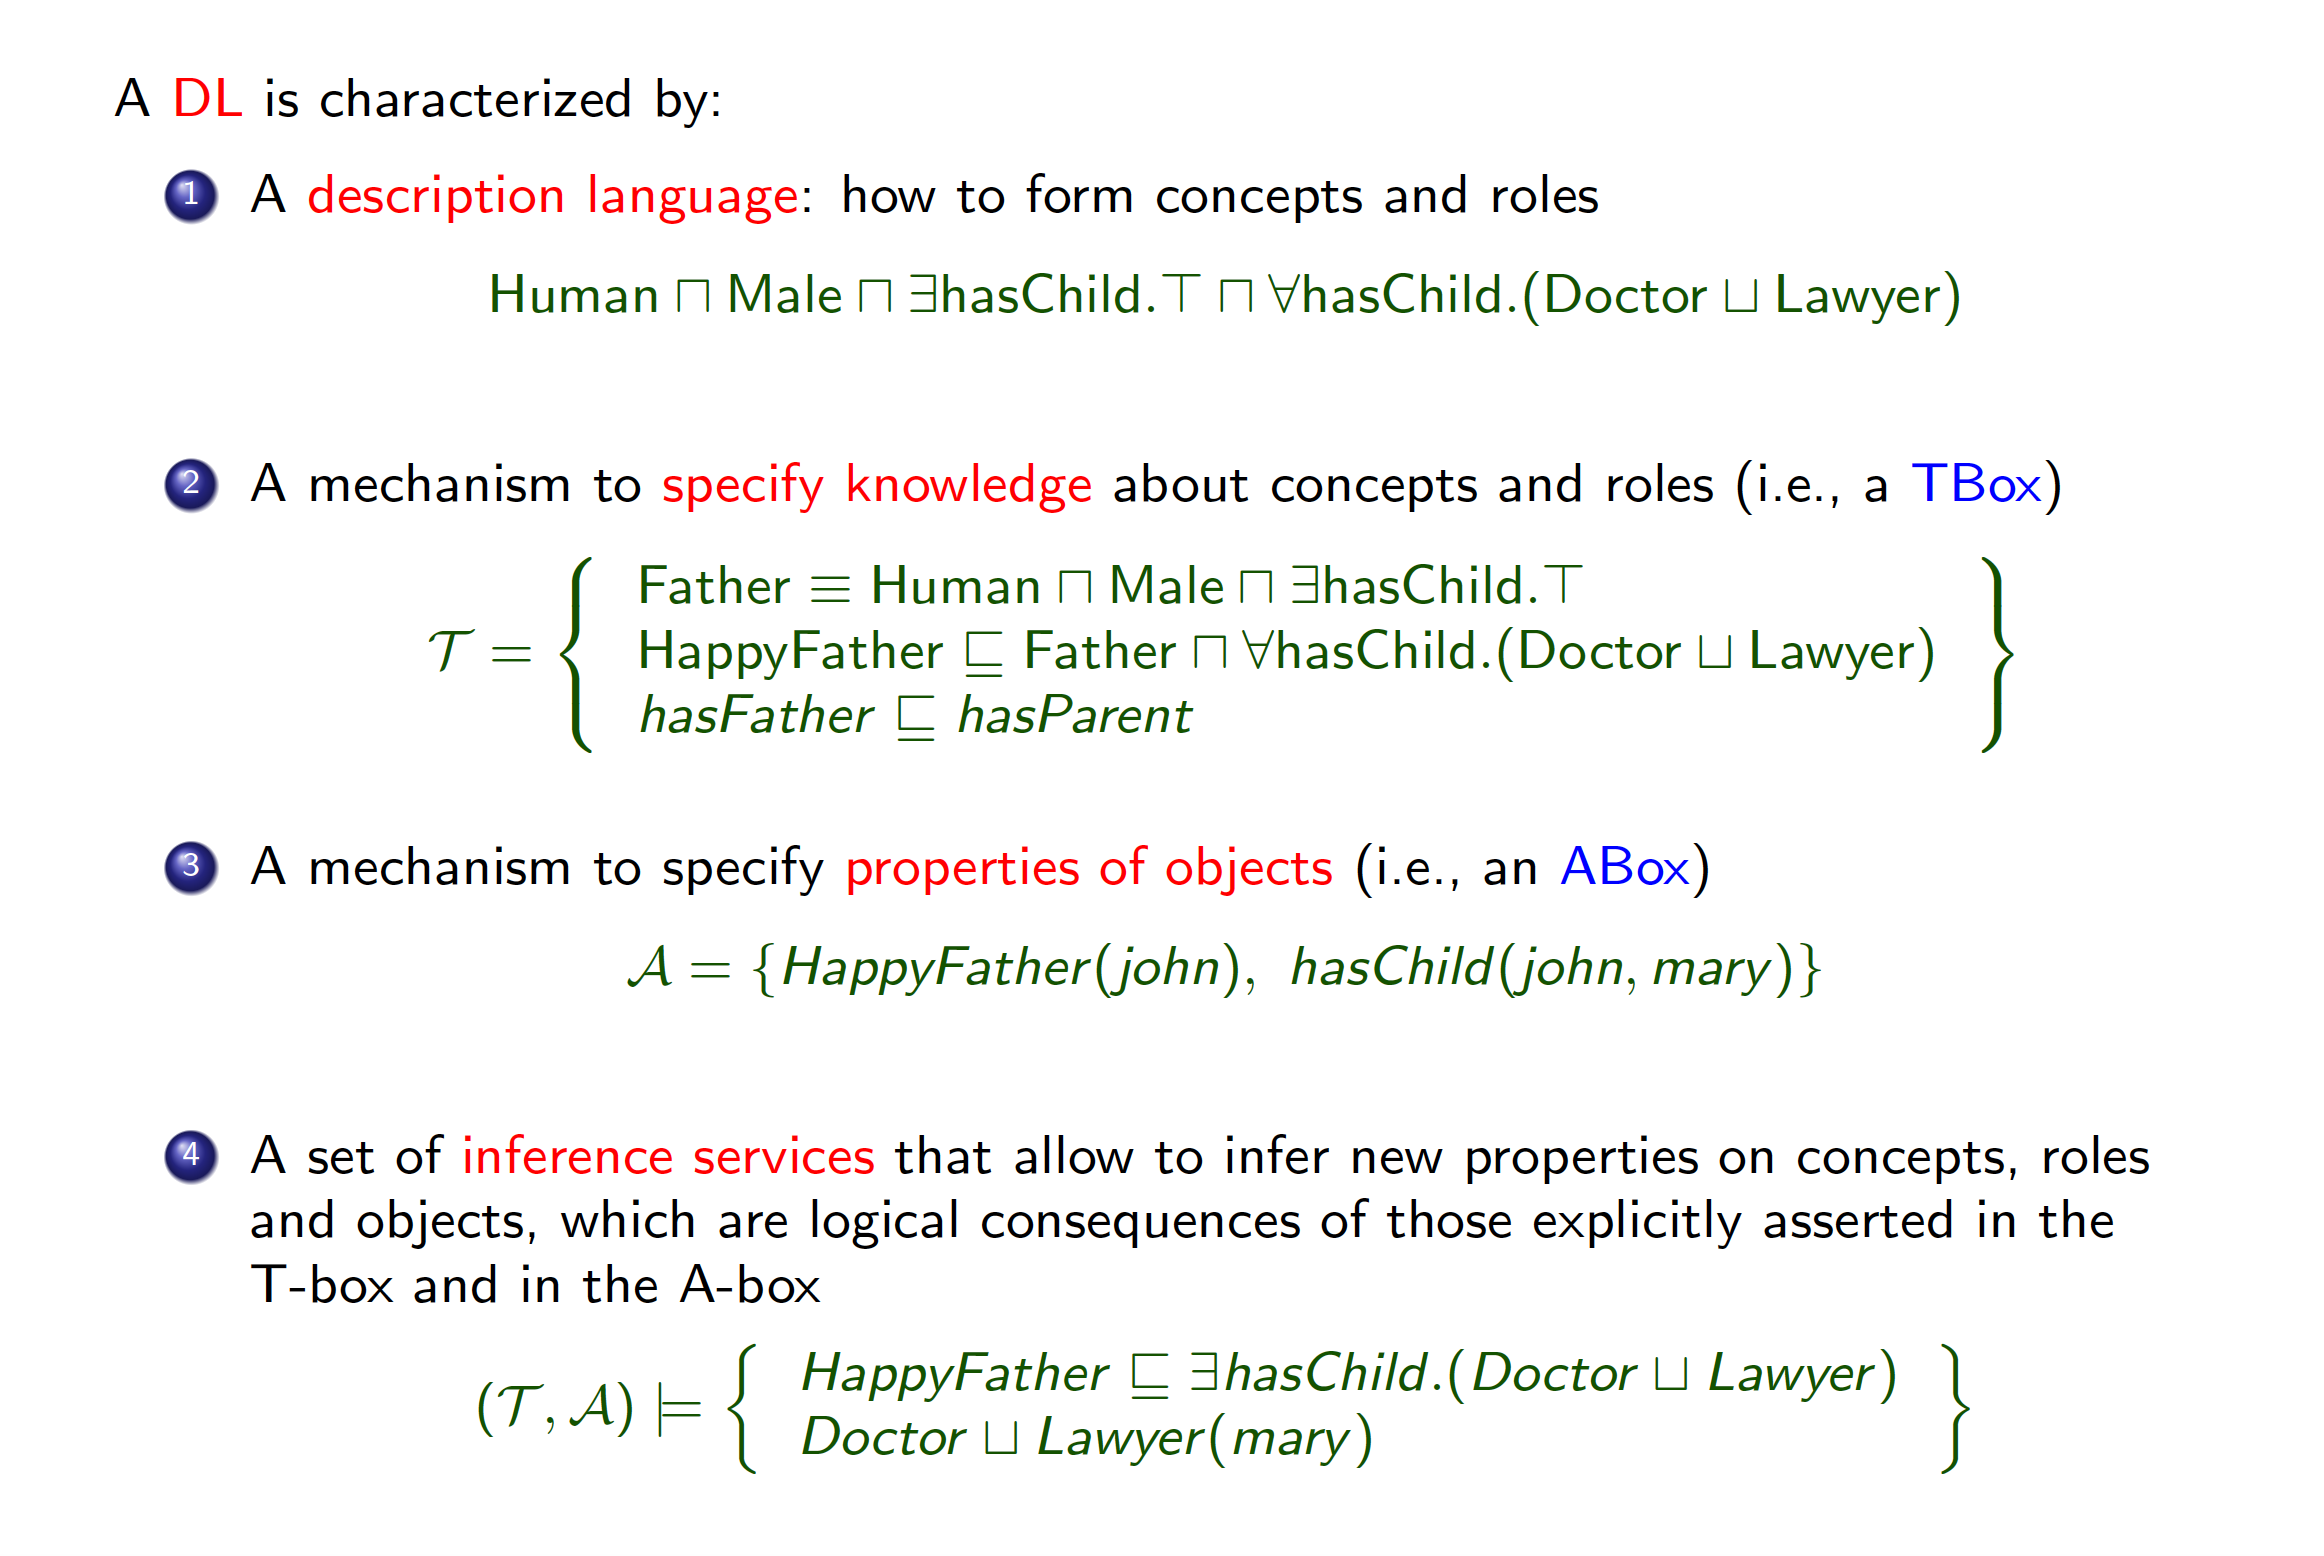
\includegraphics[scale=0.3]{Figures/DL.png}
\end{frame}


\begin{frame}
 \frametitle{Description logics : the description language}


\begin{block}{Syntaxe}
 \begin{itemize}
 \footnotesize
 \item \emph{Signature} :  un ensemble de noms de concepts, de noms de rôles et d'individus :  $\Sigma:=(\NC{}, \NR,\mathcal{N}_{\mathcal{I}})$.
 \item Descriptions de concepts :
 \[
 C::=\underbrace{\underbrace{A \mid (C \sqcap C) \mid (\exists r.C) \mid \top}_{\mathcal{EL}{}} \mid (C \sqcup C) \mid (\forall r.C) \mid \neg C  \mid \bot \mid}_{\mathcal{ALC}} \mid \{a\}  \cdots  
 \]
 avec A un concept atomique, $a$ un individu et $r$ un rôle atomique
 \end{itemize}
\end{block}
 


 \end{frame} 

\begin{frame}
\frametitle{Description logics : the description language}

\begin{block}{Sémantique}
\scriptsize
An \textcolor{red}{interpretation} $\I=\langle\Delta^\I, .^\I \rangle$
\begin{itemize}
\scriptsize
\item $\Delta^\I:$ a \textcolor{red}{non-empty set}, the domain of interpretation
\item $.^\I: $ an \textcolor{red}{interpretation function}, which assigns to :
\begin{itemize}
\footnotesize
\item  every atomic concept $A \in N_C$, a set $A^\I \subseteq \Delta^\I$,
\item every atomic role $r \in N_R$, a binary relation $r^\I \subseteq \Delta^\I \times \Delta^\I$.
\item  every individual $o \in \mathcal{N}_{\mathcal{I}} $ is mapped into an element of the interpretation domain, $o^\I \in \Delta^\I$
\end{itemize}
\end{itemize}
\end{block}

\begin{block}{Extension to concept descriptions}
\scriptsize
\[
\begin{aligned}
\top^\I &= \Delta^\I \\
 \bot^\I &=\emptyset\\
(\neg C)^\I &= \Delta^\I \setminus C^\I\\
( C \sqcap D)^\I &= C^\I \cap D^\I\\
( C \sqcup D)^\I &= C^\I \cup D^\I\\
(\forall r.C)^\I &= \{a \in \Delta^\I \mid \forall b. (a,b)\in r^\I \rightarrow b \in C^\I\}\\
(\exists r.C)^\I &= \{a \in \Delta^\I \mid \exists b. (a,b)\in r^\I \wedge b \in C^\I\}\\
%(\exists r.C)^\I &= \{a \in \Delta^\I \mid \forall b. (a,b)\in r^\I \and b \in C^\I\}
\end{aligned}
\]
\end{block}
\end{frame}



 
 
  \begin{frame}
 \frametitle{Description logics : the description language}
  
  
  
  
   \vspace{-0.15cm}
\begin{block}{Subsomption, équivalence}
 \begin{itemize}
 \item $C$ est \emph{subsommé} par $D$ ($C\sqsubseteq D$) si $C^\I \subseteq D^\I$ pour toute
interprétation $\I$ (ex: $\mathsf{Musician}\sqsubseteq\mathsf{Artist}$).
\item $C$ et $D$ sont \emph{équivalents} ($C \equiv D$) si $C^\I = D^\I$ pour toute
interprétation $\I$.
 \end{itemize}
 \end{block}
  \vspace{-0.15cm}
 \begin{block}{Base de connaissances (ou théorie)}
 
$\mathcal{K}=\{\mathcal{T},\mathcal{A}\}$, $\mathcal{T}$ un ensemble d'axiomes (ex: $C\sqsubseteq D, C\equiv D$) et $\mathcal{A}$ un ensemble d'assertions (ex: $a:C, (a,b):R$)
 
 \end{block}
\end{frame}


\begin{frame}
\frametitle{Description logics : satisfiability }

\begin{block}{Satisfaction relation $\models$}
\begin{itemize}
    \item $\I \models (C\sqsubseteq D) \Leftrightarrow C^\I \subseteq D^\I$
    \item $\I \models (C\equiv D)  \Leftrightarrow C^\I \equiv D^\I$
    \item $\I \models (C(a))  \Leftrightarrow a^\I \in C^\I$    
    \item ...
\end{itemize}
\end{block}
A concept C is satisfiable if there is an interpretation $\I$, such that $ C^\I \neq \emptyset$
\end{frame}





\begin{frame}
\frametitle{Description logics : models }
\begin{block}{}
\begin{itemize}
\footnotesize
\item An interpretation $\I$ satisfies a GCI $C \sqsubseteq D$ iff $C^\I \subseteq D^\I$
\[
\I \models (C\sqsubseteq D) \Leftrightarrow C^\I \subseteq D^\I
\]
\item An interpretation $\I$ satisfies an equality $C \equiv D$ if $C^\I \equiv D^\I$
\[
\I \models (C\equiv D)  \Leftrightarrow C^\I \equiv D^\I
\]
\item The interpretation $\I$  is a \textcolor{red}{model} of a TBox $\mathcal{T}$ iff it satisfies all the GCIs in $\mathcal{T}$
\item Two TBoxes are \textcolor{red}{equivalent} if they have the same model.
\item $\I$ is a model of the ABox $\A$ if it satisfies all its assertions:

\end{itemize}
\end{block}

\end{frame}






\begin{frame}
\frametitle{Description logics: reasoning services}
\framesubtitle{Terminological reasoning}
\begin{block}{Satisfiability}
\footnotesize
$C$ is satisfiable w.r.t. a TBox $\T$ iff $C^\I \neq \emptyset$ for some model $\I$ of $\T$.
\end{block}

\begin{block}{Subsumption}
\footnotesize
$C$ is subsumed by $D$ w.r.t. a TBox $\T$ ($C \sqsubseteq_\T D$) iff $C^\I \subseteq D^\I$ for all  models $\I$ of $\T$.
\end{block}

\begin{block}{Equivalence}
\footnotesize
$C$ is equivalent to $D$ w.r.t. a TBox $\T$ ($C \equiv_\T D$) iff $C^\I = D^\I$ for all  models $\I$ of $\T$.
\end{block}

\begin{block}{Disjointness}
\footnotesize
Two concepts $C$ and $D$ are disjoint with respect to $\T$ if $C^\I \cap D^\I = \emptyset$ for every model $\I$ of $\T$.
\end{block}


\vspace{2cm}
\hfill $\sqsubseteq_\T$ is a pre-order (reflexive and transitive).


\end{frame}


\begin{frame}
\frametitle{Description logics: reasoning services}
\framesubtitle{Assertional reasoning}
\footnotesize
Let $\K=(\T,\A)$ be an ontology. 
\begin{block}{Consistency}
\footnotesize
$\A$ is consistent with respect to a TBox $\T$, if there is an interpretation that is a model of both $\A$ and $\T$.
\end{block}
\begin{block}{Instance checking}
\footnotesize
$a$ is an instance of $C$ w.r.t. $\T$ iff $a^\I \in C^\I$ for all models $\I$ of $\T$. We also write $\A\models C(a)$. The same holds for roles.
\end{block}
\begin{block}{Retrieval problem}
\footnotesize
Given an ABox $\A$ and a concept $C$, find all individuals $a$ such that $\A\models C(a)$.
\end{block}
\begin{block}{Realization problem (dual to the retrieval problem)}
\footnotesize
 Given an individual $a$ and a set of concepts, find {\em the most specific concepts} (msc) $C$ from the set such that $\A \models C(a)$. The mscs are the concepts that are minimal with respect to the subsumption ordering $\sqsubseteq$.
\end{block}
\end{frame}




\begin{frame}{Dans le papier : logiques de description $\mathcal{E}\mathcal{L}^{++}$}
\begin{block}{Syntaxe}
 \begin{itemize}
 \item \emph{Signature} :  un ensemble de noms de concepts et de noms de rôles et d'individus  $\Sigma:=(\NC{}, $\NR$, \mathcal{N}_I)$.
 \item Descriptions de concepts :
 \[
A \mid (C \sqcap D) \mid (\exists r.C) \mid \top  \mid \bot \mid \{a\}
 \]
 %\item $\Lmc$: a logic, $\C{\Lmc}$: set of concepts.
% \item Subsumption: $C\sqsubseteq D$, equivalence: $C \equiv D$.
 \end{itemize}
\end{block}

\begin{block}{Ontologie}
\[
\mathcal{O} = \mathcal{T} \sqcup \mathcal{A}
\]
\end{block}

\begin{figure}
    \centering
    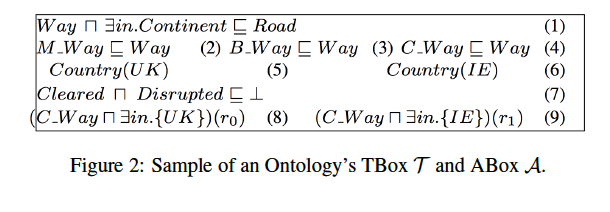
\includegraphics[scale=0.4]{Figures/Tboxexample.png}
\end{figure}

\end{frame}


\begin{frame}{Entailment closure}

Given an Ontology $\mathcal{T} \sqcup \mathcal{A}$, we consider the closure of atomic ABox entailment, $\mathcal{G}(\mathcal{T} \sqcup \mathcal{A})$ as  $\{g | \mathcal{T} \sqcup \mathcal{A} \models g \}$ where $g$ represents an atomic concept assertion $A(b)$ or and atomic role assertions $r(a,b)$ involving only named concepts, named roles and named individuals.

\end{frame}


\section[Formalisation]{Formalisation des domaines avec des ontologies}


\begin{frame}{Contribution}
Formalisation des domaines d'apprentissage et de la tâche d'apprentissage avec les DLs
\begin{block}{Définition 1 : Learning Sample Ontology (LSO) [Chen et al, 2018]}
\begin{itemize}
\item Ontologie $\mathcal{O} =\langle\langle \mathcal{T}, \mathcal{A} \rangle, S \rangle$ : ontologie annotée avec des paires de propriétés-valeurs.
\item Permet de représenter la notion de dataset : les entrées.
\end{itemize}
\end{block}
\begin{figure}
    \centering
    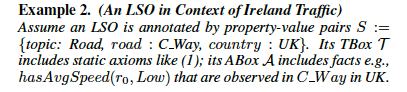
\includegraphics[scale=0.5]{Figures/LSO.png}
\end{figure}

\end{frame}

\begin{frame}{Contribution}
\begin{block}{Définition 2 : Learning Domain and Target Entailment}
\begin{itemize}
    \item Learning Domain : $\mathcal{D}=\langle \mathbb{O}, \mathcal{G}^{\mathcal{Y}} \rangle $ : a set of LSOs that share the same TBox $ \mathcal{T}$ and target entailments $\mathcal{G}^{\mathcal{Y}}$
\end{itemize}

\end{block}
\end{frame}


\begin{frame}{Contribution}
\begin{block}{Définition 3 : Semantic learning task}
 \centering
    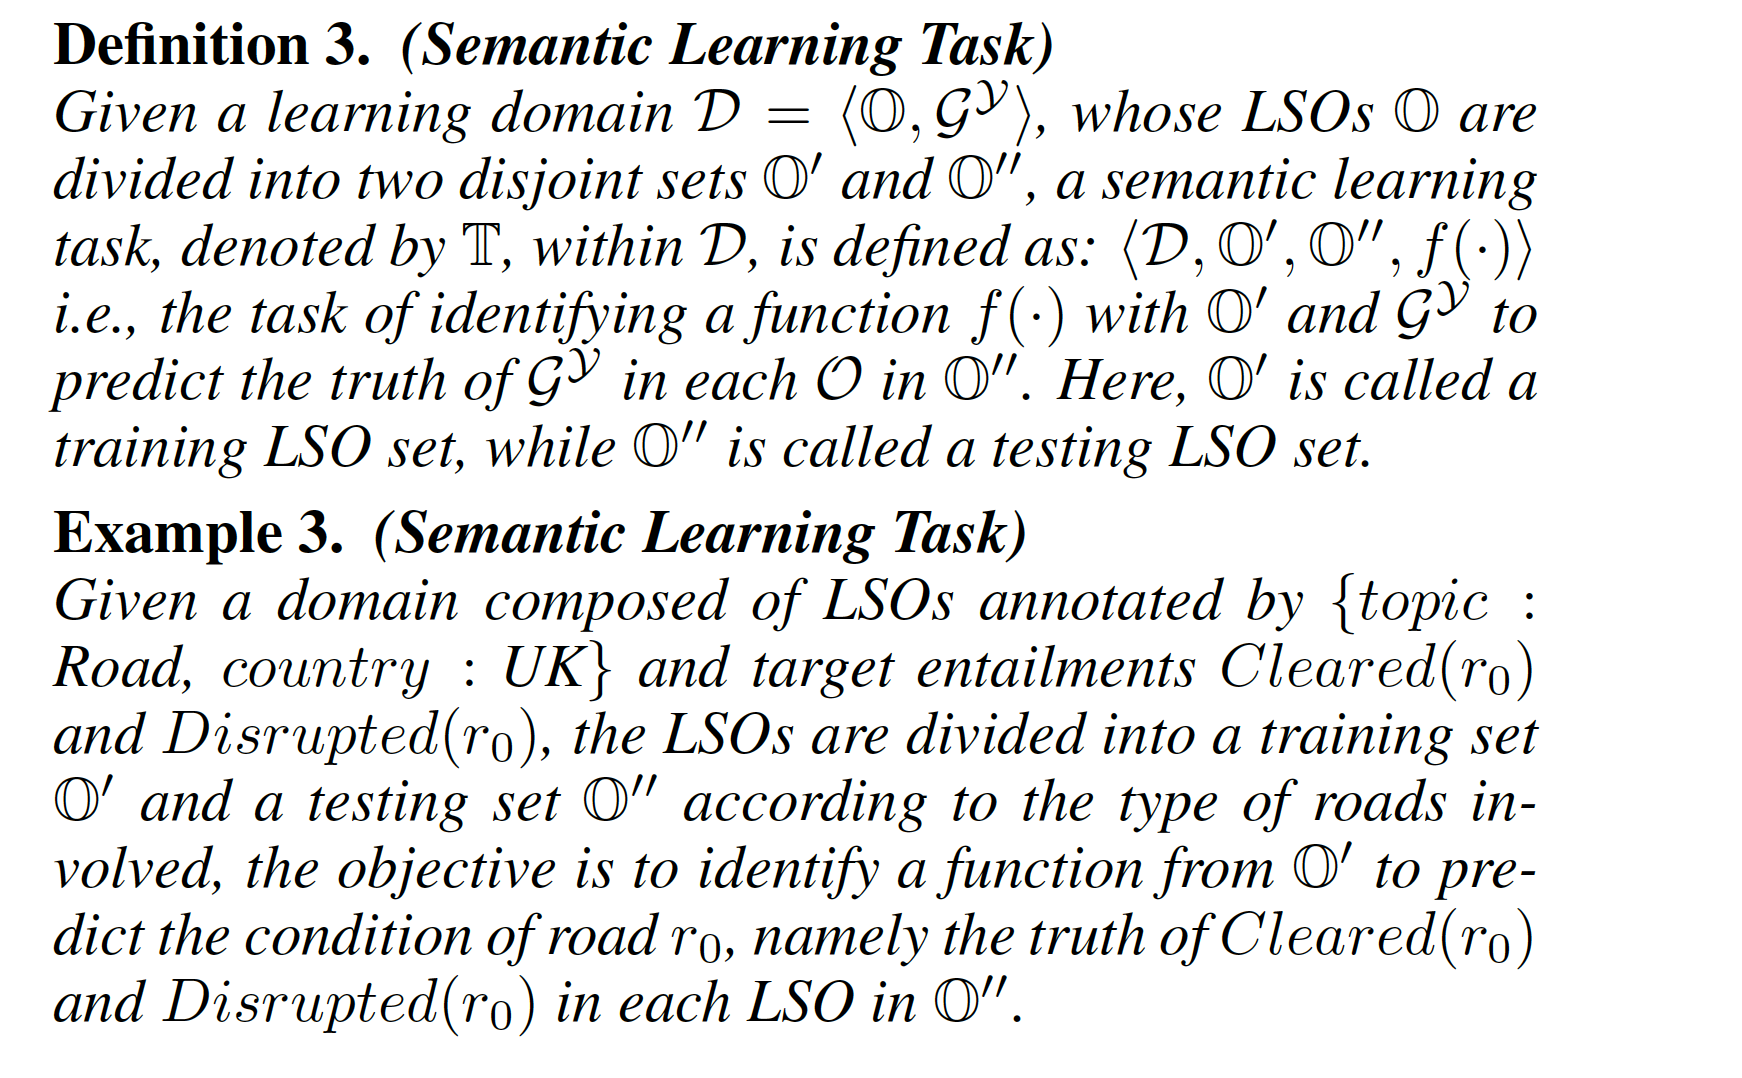
\includegraphics[scale=0.3]{Figures/SLT.png}

\end{block}
\end{frame}


\begin{frame}{Contribution}
\begin{block}{Définition 4 : Transfer Learning accross domains}
 \centering
    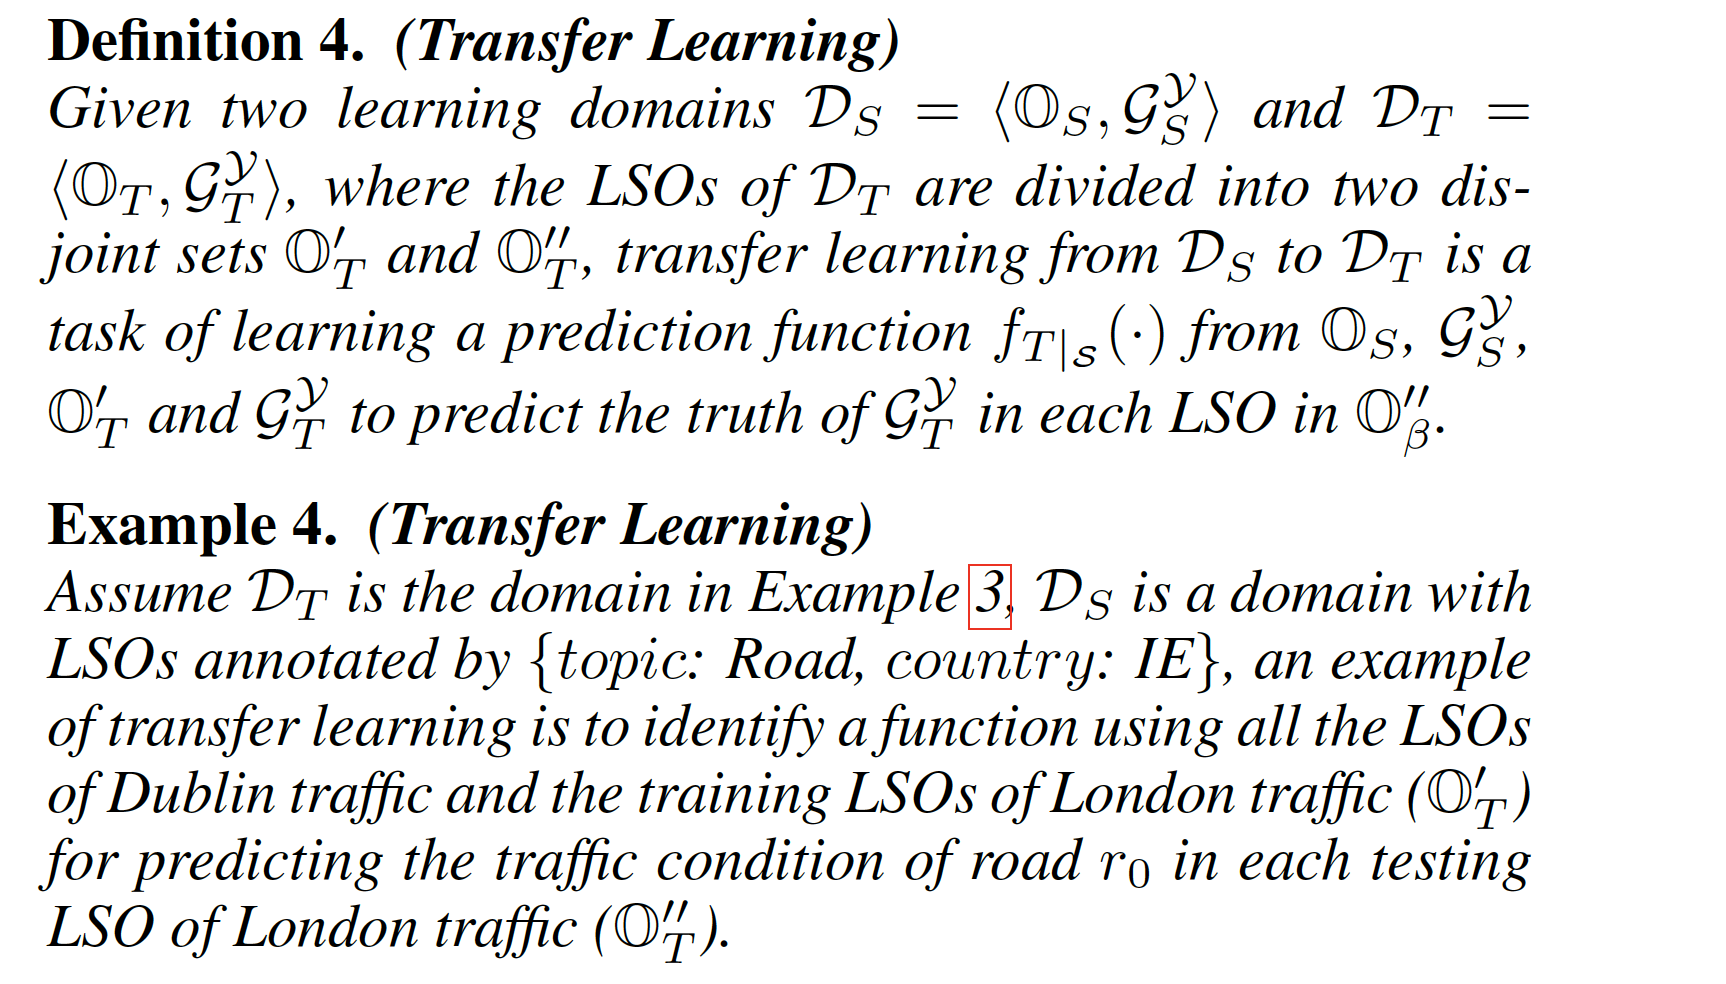
\includegraphics[scale=0.3]{Figures/TL.png}

\end{block}
\end{frame}


\begin{frame}{Contribution}
\begin{block}{Idée}
\begin{itemize}
    \item Utiliser les ontologies pour guider le transfert.
    \item $\rightarrow$ étude de la variabilité des ABOx entailments.
\end{itemize}
\end{block}

\end{frame}

\begin{frame}{Contribution}
\begin{block}{Définition 5 : Entailment-based domain variability}
 \centering
    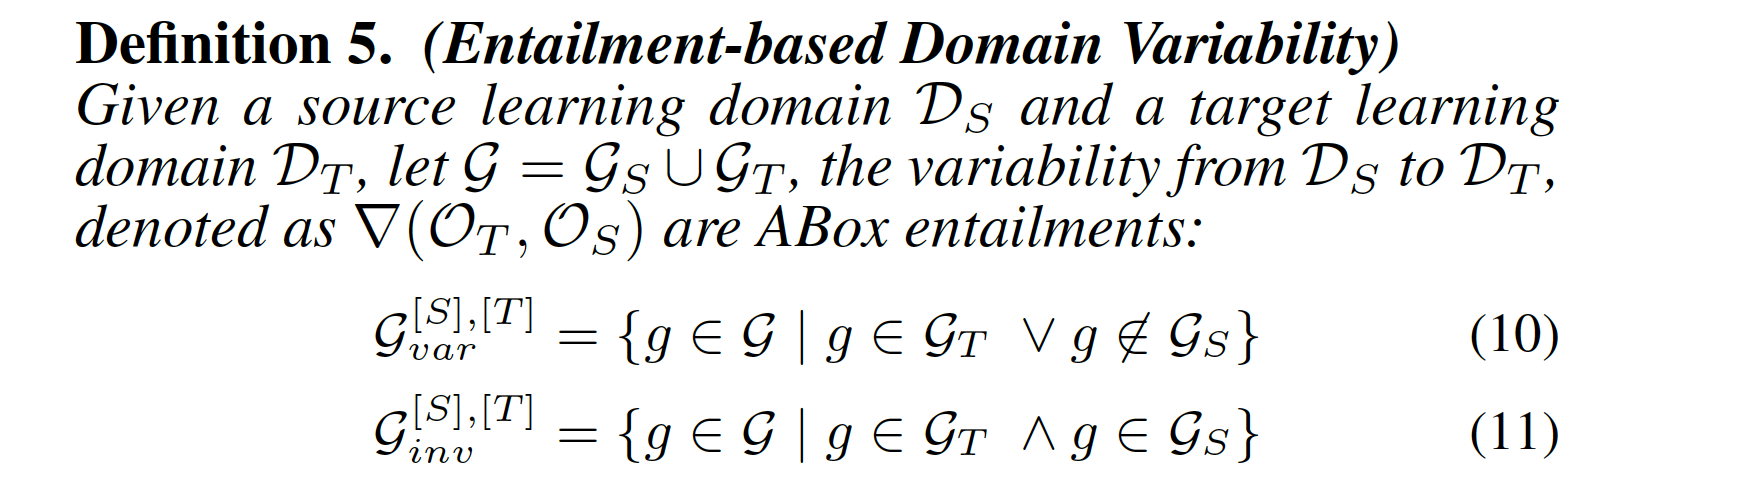
\includegraphics[scale=0.3]{Figures/variability.png}
\end{block}
\begin{itemize}
    \item (11) exprime la connaissance invariante
    \item (10) exprime la connaissance variante
\end{itemize}
Au niveau d'un domaine.
\end{frame}

\begin{frame}{Tranferability}
\begin{block}{Variability of semantic learning tasks}
 \centering
    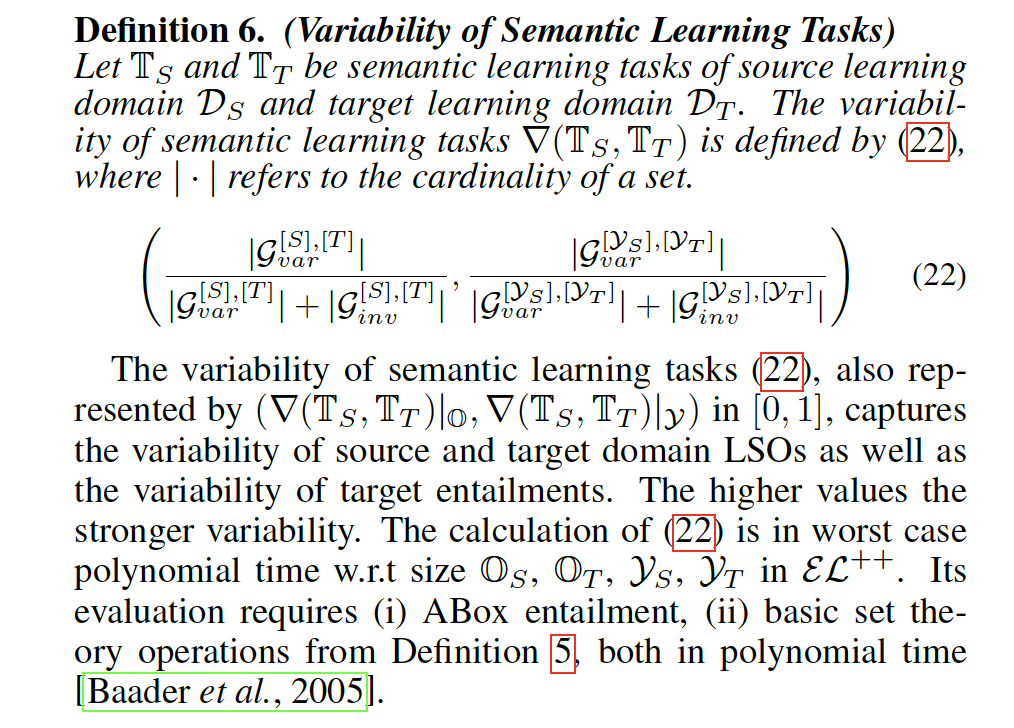
\includegraphics[scale=0.4]{Figures/VSLT.png}
\end{block}
\end{frame}


\begin{frame}{Tranferability}
\begin{block}{Semantic transferability : When to transfer ?}
\footnotesize
Définie comme l'existence de connaissance capturée par les ABox entailements dans la source et qui ont un effet positif sur la qualité de la prédiction sur la tâche cible.

 \centering
    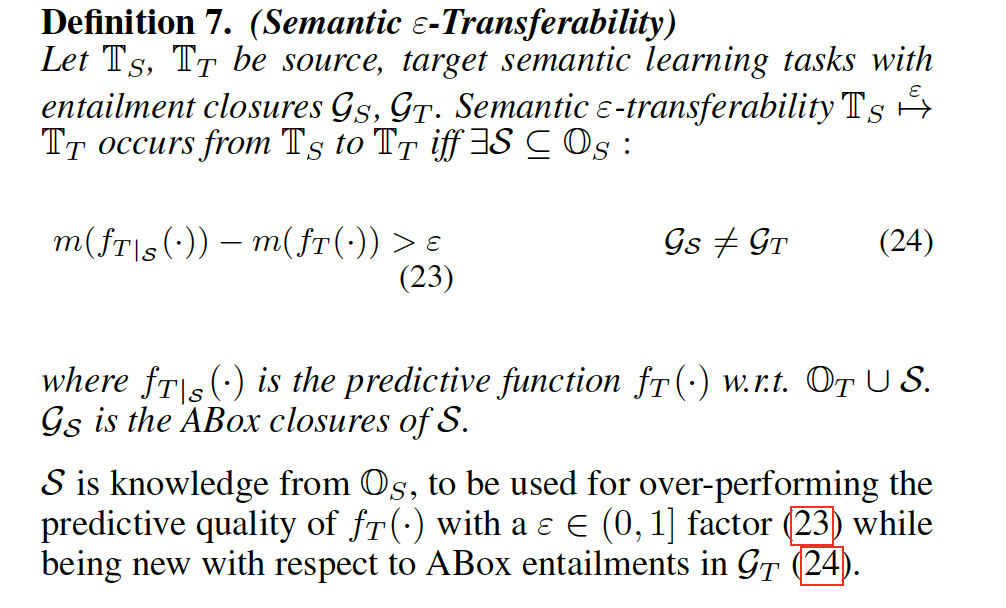
\includegraphics[scale=0.4]{Figures/epsilon.png}
\end{block}
\end{frame}


\begin{frame}{Tranferability}
\begin{block}{Semantic transferability :Exemple}

 \centering
    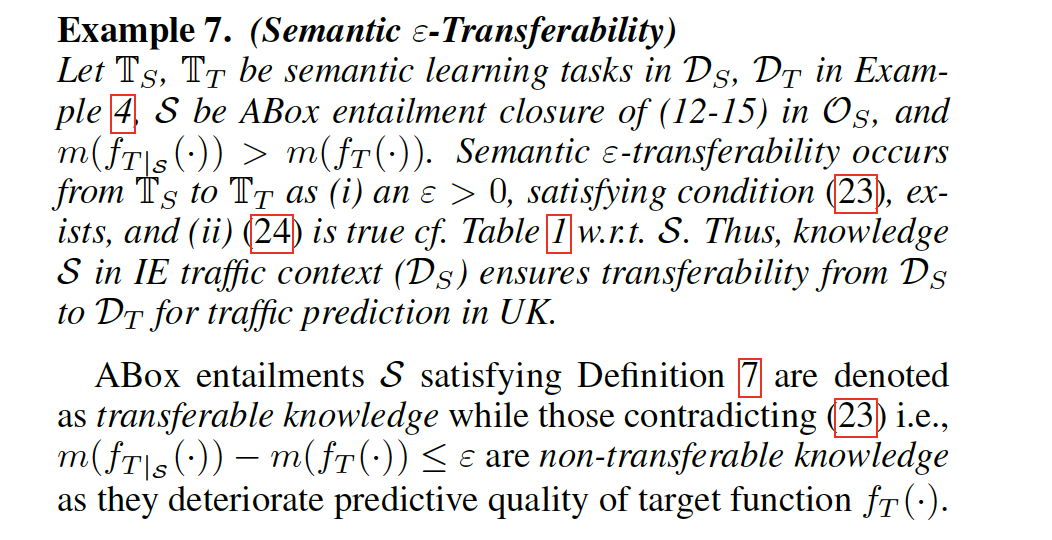
\includegraphics[scale=0.4]{Figures/epsilon2.png}
\end{block}
\end{frame}

\begin{frame}{Tranferability}
\begin{block}{Consistent transferable knowledge}

 \centering
    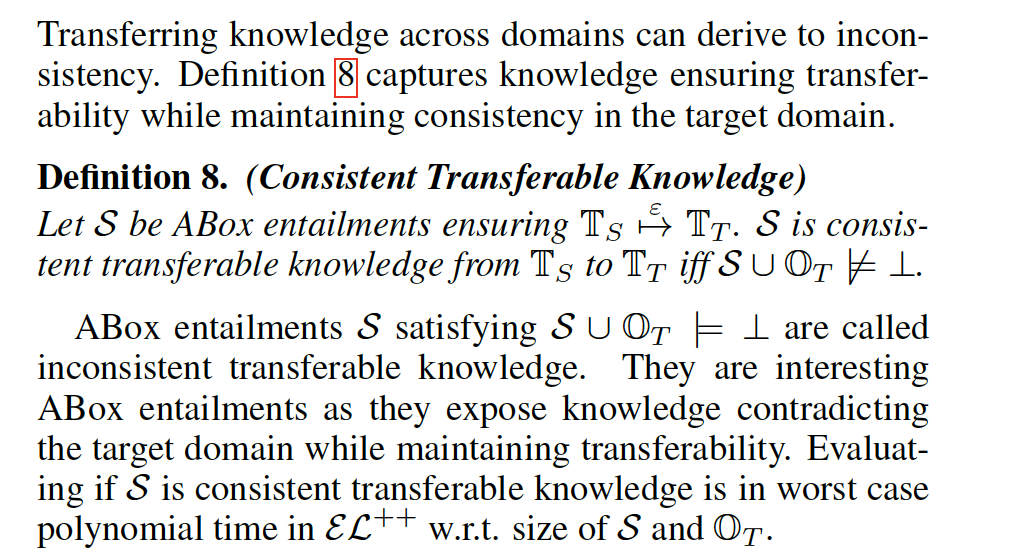
\includegraphics[scale=0.4]{Figures/consistent.png}
\end{block}
\end{frame}

\begin{frame}{Semantic Tranfer Learning}
\begin{block}{Semantic  Embedding : How to transfer ? }
3 vecteurs : transferability, consistency, variability

 \centering
    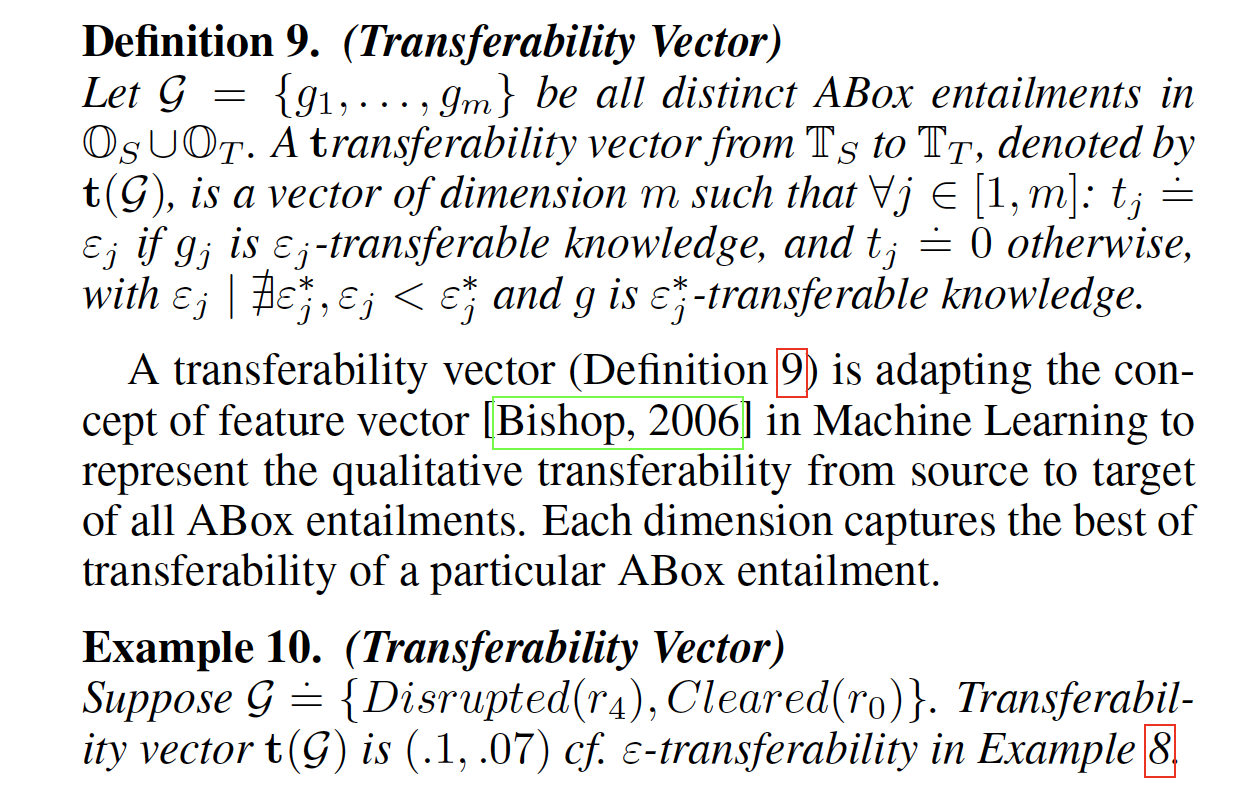
\includegraphics[scale=0.4]{Figures/tv.png}
\end{block}
\end{frame}

\begin{frame}{Semantic Tranfer Learning}
\begin{block}{Semantic  Embedding : How to transfer ? }
3 vecteurs : transferability, consistency, variability

 \centering
    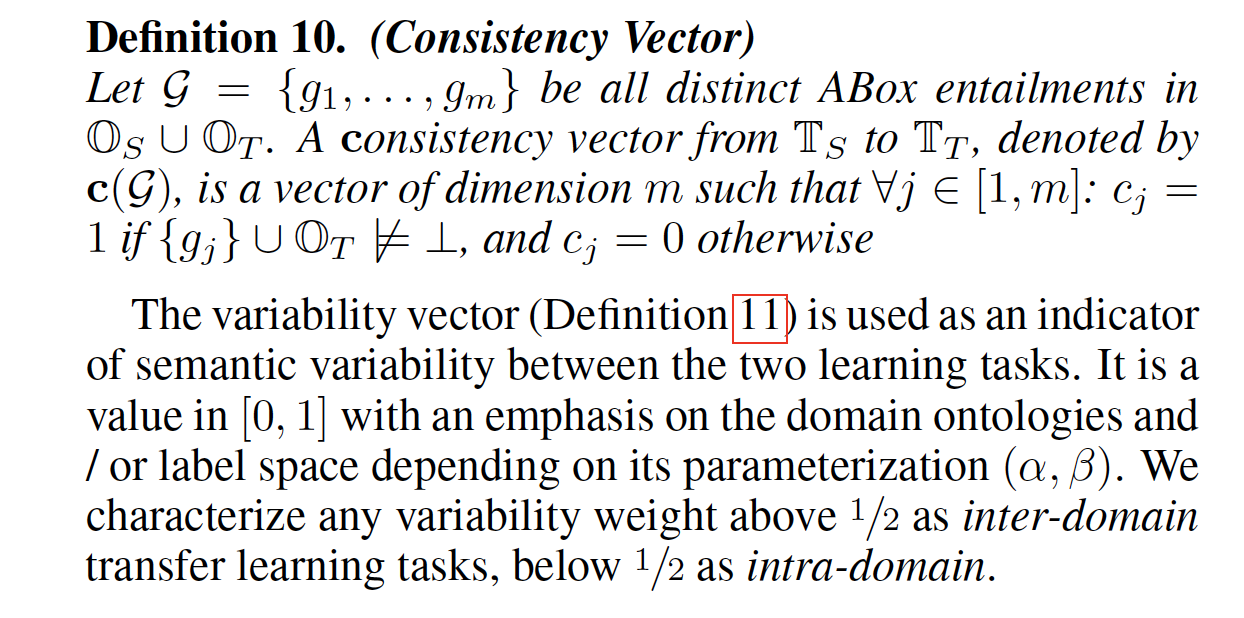
\includegraphics[scale=0.4]{Figures/cv.png}
\end{block}
\end{frame}



\begin{frame}{Semantic Tranfer Learning}
\begin{block}{Semantic  Embedding : How to transfer ? }
3 vecteurs : transferability, consistency, variability

 \centering
    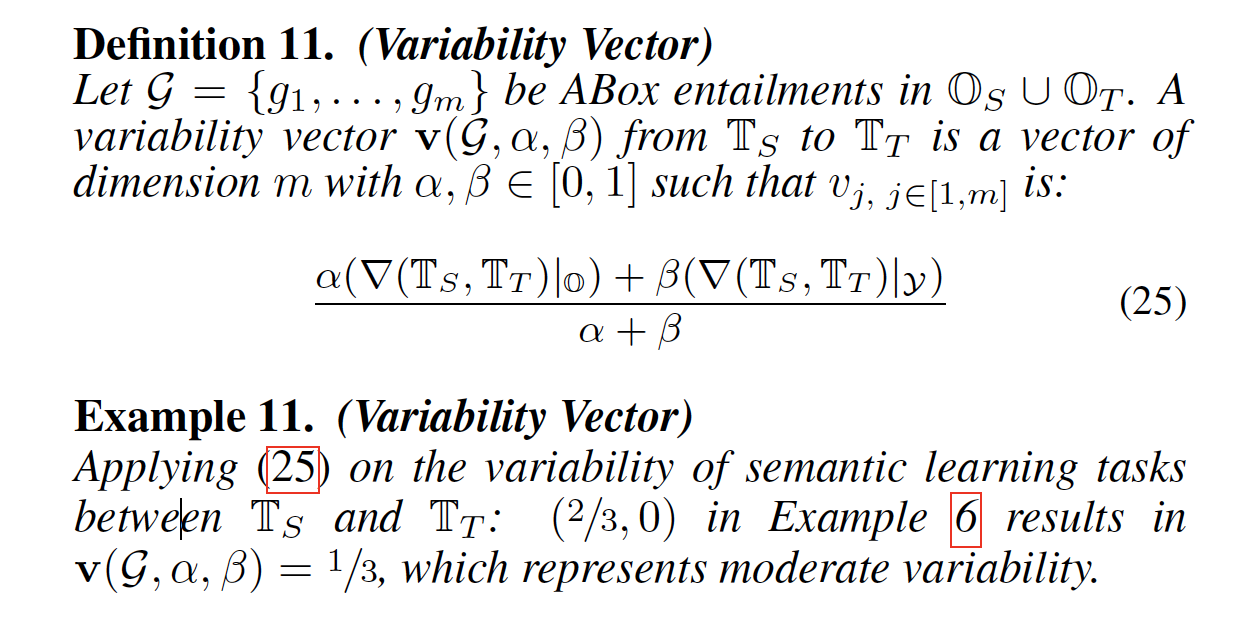
\includegraphics[scale=0.4]{Figures/vv.png}
\end{block}
\end{frame}


\begin{frame}{Boosting for semantic transfer leaning}
Voir algorithme sur le papier.
\end{frame}

\begin{frame}{Expérimentations}
\begin{itemize}
    \item Evaluation sur 2 tâches de Intra-transfer learning  et une inter-domain
    \begin{itemize}
        \item IBH : air quality forecasting : Beijing to Hangzhou
        \item ILD : traffic condition prediction : London to Dublin
        \item ILB : traffic condition in London to air quality in Beijing
        
    \end{itemize}
\end{itemize}
\end{frame}

\begin{frame}{Résultats}

 \centering
    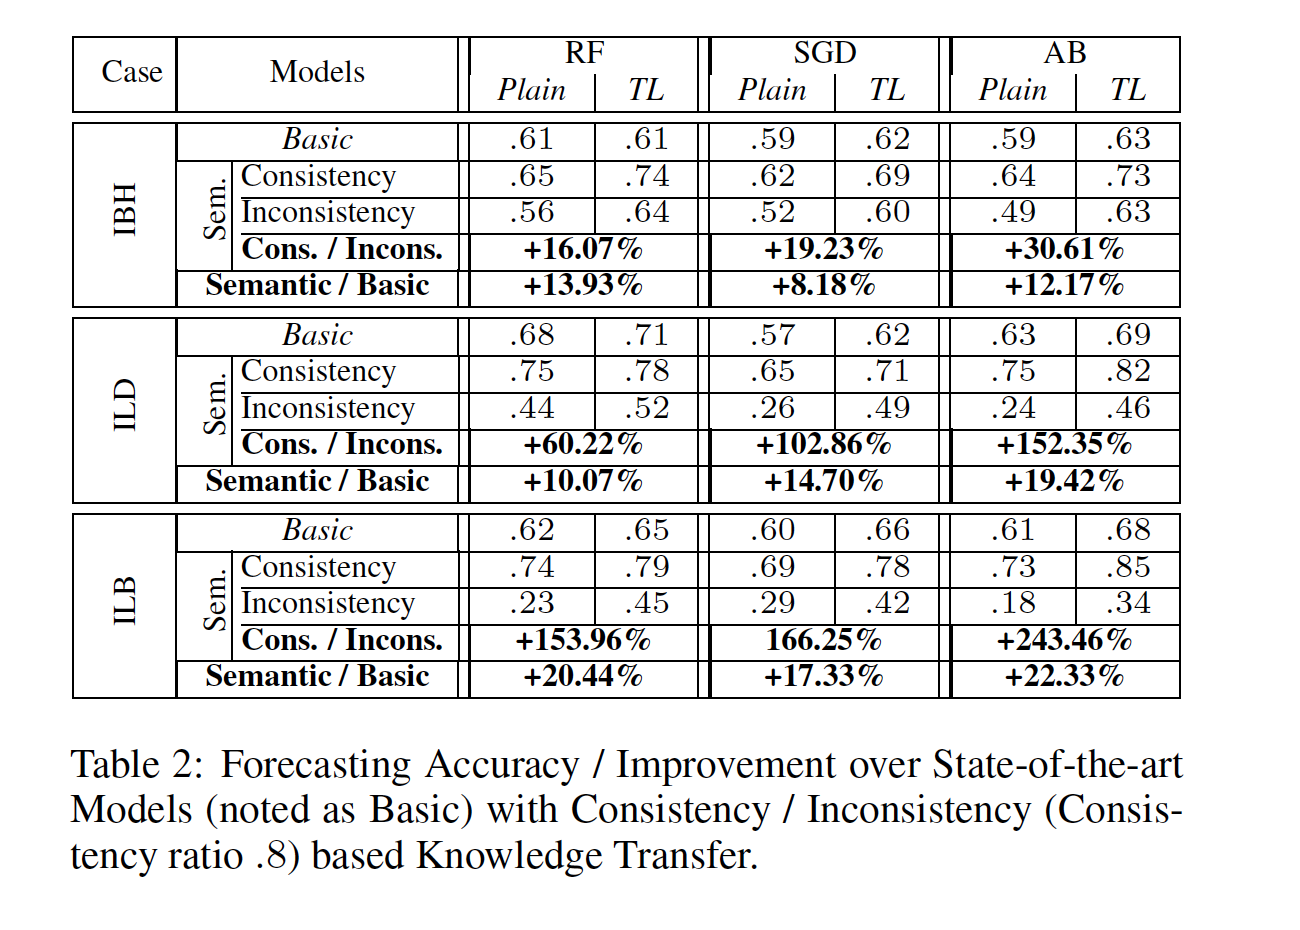
\includegraphics[scale=0.4]{Figures/result.png}

\end{frame}


\begin{frame}{Discussion}
\begin{itemize}
    \item Un travail plus approfondi, en se basant sur les exemples et une éventuelle implémentation reste à faire.
    \item Travail intéressant surtout concernant l'utilisation de raisonnements ontologiques pour sélectionner les exemples transférables (lien avec AL par exemple)
    \item Travail sur les liens entre les différents paradigmes : consistency... : ijcai 2021 (mi janvier ?)
    
\end{itemize}


\end{frame}


%\begin{frame}{Knowledge Transfer with Interactive Learning of Semantic Relationship}
%\begin{figure}
%    \centering
%    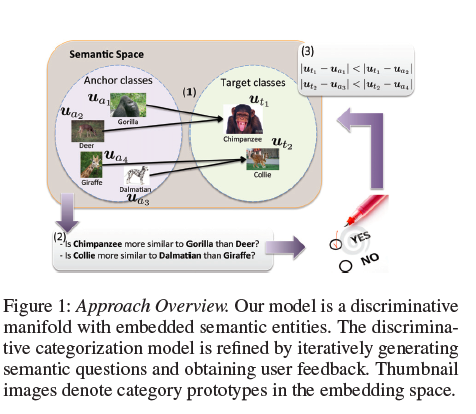
\includegraphics[scale=0.5]{Figures/choi.png}
%\end{figure}
%\end{frame}

%\begin{frame}{Transfer Learning for Deep Learning on Graph-Structured Data}
%\begin{figure}
%    \centering
%    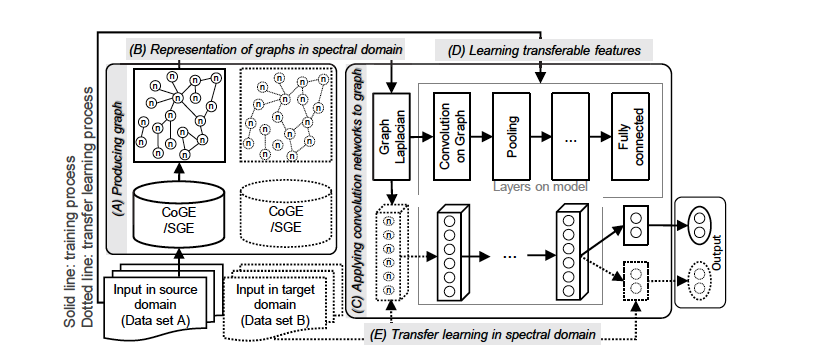
\includegraphics[scale=0.4]{Figures/lee.png}
%\end{figure}
%\end{frame}


\end{document}
